% Copyright 2004 by Till Tantau <tantau@users.sourceforge.net>.
%
% In principle, this file can be redistributed and/or modified under
% the terms of the GNU Public License, version 2.
%
% However, this file is supposed to be a template to be modified
% for your own needs. For this reason, if you use this file as a
% template and not specifically distribute it as part of a another
% package/program, I grant the extra permission to freely copy and
% modify this file as you see fit and even to delete this copyright
% notice. 

\documentclass{beamer}

% There are many different themes available for Beamer. A comprehensive
% list with examples is given here:
% http://deic.uab.es/~iblanes/beamer_gallery/index_by_theme.html
% You can uncomment the themes below if you would like to use a different
% one:
%\usetheme{AnnArbor}
%\usetheme{Antibes}
%\usetheme{Bergen}
%\usetheme{Berkeley}
%\usetheme{Berlin}
%\usetheme{Boadilla}
%\usetheme{boxes}
%\usetheme{CambridgeUS}
%\usetheme{Copenhagen}
%\usetheme{Darmstadt}
%\usetheme{default}
%\usetheme{Frankfurt}
%\usetheme{Goettingen}
%\usetheme{Hannover}
%\usetheme{Ilmenau}
%\usetheme{JuanLesPins}
%\usetheme{Luebeck}
\usetheme{Madrid}
\usecolortheme{beaver}
%\usetheme{Malmoe}
%\usetheme{Marburg}
%\usetheme{Montpellier}
%\usetheme{PaloAlto}
%\usetheme{Pittsburgh}
%\usetheme{Rochester}
%\usetheme{Singapore}
%\usetheme{Szeged}
%\usetheme{Warsaw}

\title{Parallel Backpropagation for Multilayer Neural Networks}

% A subtitle is optional and this may be deleted
\author[]{Palash Goyal\inst{1}
\and Nitin Kamra\inst{1} \and
        Sungyong Seo\inst{1} \and Vasileios Zois\inst{1}}
% - Give the names in the same order as the appear in the paper.
% - Use the \inst{?} command only if the authors have different
%   affiliation.

%\logo{\includegraphics[height=0.8cm]{target.jpg}\vspace{225pt}}

\institute[University of Southern California] % (optional, but mostly needed)
{
  \inst{1}%
  Department of Computer Science\\
  University of Southern California
 }
% - Use the \inst command only if there are several affiliations.
% - Keep it simple, no one is interested in your street address.

%\date{Conference Name, 2013}
% - Either use conference name or its abbreviation.
% - Not really informative to the audience, more for people (including
%   yourself) who are reading the slides online

%\subject{Theoretical Computer Science}
% This is only inserted into the PDF information catalog. Can be left
% out. 

% If you have a file called "university-logo-filename.xxx", where xxx
% is a graphic format that can be processed by latex or pdflatex,
% resp., then you can add a logo as follows:

% \pgfdeclareimage[height=0.5cm]{university-logo}{university-logo-filename}
% \logo{\pgfuseimage{university-logo}}

% Delete this, if you do not want the table of contents to pop up at
% the beginning of each subsection:
\AtBeginSubsection[]
{
  \begin{frame}<beamer>{Outline}
    \tableofcontents[currentsection,currentsubsection]
  \end{frame}
}

% Let's get started
\begin{document}

\begin{frame}
  \titlepage
\end{frame}

\begin{frame}{Outline}
  \tableofcontents
  % You might wish to add the option [pausesections]
\end{frame}

% Section and subsections will appear in the presentation overview
% and table of contents.



  \section{Introduction}
\label{Intro}

Artificial neural networks are powerful machine learning tools used in many applications including but not limited to search engines, spam and fraud detection, image classification, diagnostic medicine applications and stock market prediction.

Prior to application, neural networks undergo a training phase which is known to be very computationally intensive. This is primarily because the prevailing neural network architectures are implemented using several hidden layers, with each one consisting of thousands to millions of neurons in order to generalize well on diverse inputs. In this case, the resulting number of parameters that need to be trained are in the order of millions.

Furthermore, achieving high accuracy requires considering a large number of training examples (usually in the order of millions). For this reason training a neural network is both a data and resource intensive operation. This calls for efforts to parallelize the training process on multi-core and while emphasizing at utilizing the maximum available bandwidth.

Currently Minibatch Gradient Descent (henceforth called MGD) is the most commonly used optimization algorithm used to train neural networks in supervised settings. It is implemented in a layerwise-recursive fashion which is termed \textit{backpropagation} in the context of neural networks.

In this paper, we have implemented parallel backpropagation to train Multi Layer Perceptrons (MLPs) for classification tasks.
The rest of the paper is organized as follows: section \ref{ProbDesc} presents a description of supervised learning tasks and neural networks as classifiers. Section \ref{BackProp} describes the conventional serial backpropagation algorithm, and an approach to parallelization using multiple threads. Section \ref{GPUBackProp} describes how to implement backpropagation on a GPU with cuda. Section \ref{Exp} describes our datasets and the experiments we performed on them. Section \ref{Results} presents our results obtained for these implementations and analyzes the speedup obtained for various network architectures and increasing problem sizes. It also presents a comparison with the same algorithms implemented using a state-of-the-art neural network library Theano. Finally, we conclude in section \ref{Future} with a discussion of potential applications and future work for this project.
   
  \section{Why mini batch?}

\begin{frame}{Gradient Descent}

\begin{itemize}
  \item{Suppose we have some training set $(x_i,y_i)$ for $i=1,\cdots,N$:}
    \begin{align*}
    \mathcal{L}_{MSE}(\theta)=\frac{1}{N}\sum_{i=1}^{N}(y_i-f(x_i;\theta))^2
    \end{align*}
    \item{Then, the parameters are updated as follow:}
        \begin{align*}
        \theta_j=\theta_j - \alpha\frac{\partial\mathcal{L}_{MSE}(\theta)}{\partial\theta_j}
        \end{align*}
        \end{itemize}
\end{frame}
        
\begin{frame}{Batch vs. Stochastic}  
  \begin{itemize}
    \item{If the gradient is computed by using whole dataset ($N$), it is Batch Gradient Descent. }
	\begin{itemize}
	\item {This is great for convex, or relatively smooth error manifolds.}
	\item{Gradient is less noisy (averaged over a large number of samples).}
	\item{For large or infinite datasets, batch gradient is impractical.}
	%\item{It is able to use optimized matrix operations to efficiently compute output and gradient over whole dataset.}
	\end{itemize}
	\item{Stochastic Gradient Descent(SGD) computes the gradient using a single example.} 	    
	\begin{itemize}
	\item {SGD works well for error manifolds that have lots of local maxima/minima because the somewhat noisy gradient helps to escape local minima into a region that hopefully is more optimal.}
%	\item{More parameters updates imply faster convergence.}
	\item {SGD may go "zig-zag" to a local minimum because of highly noisy gradient.} 
	\end{itemize}
  \end{itemize}
\end{frame}



\begin{frame}{Alternative: Mini Batch}
  \begin{itemize}
    \item{Mini Batch Gradient Descent (MGD) is to compute the gradient against more than one training example at each step.}
    \item{$M$ is the mini batch size.}
  \end{itemize}
  \begin{align*}
    & \mathcal{L}^k_{MSE}(\theta)=\frac{1}{M}\sum_{i=s_k}^{s_k+M}(y_i-f(x_i;\theta))^2\\    
       & \theta_k=\theta_k - \alpha\frac{\partial\mathcal{L}^k_{MSE}(\theta)}{\partial\theta_k}
    \end{align*}
    \begin{itemize}
    \item{Parallelization : Distributing training examples across various processors and letting them compute a partial gradient over their own training examples.}
%        \item{Computing the gradient for many cases simultaneously uses matrix-­‐matrix multiplies which are very efficient, especially on GPUs.}
    \end{itemize}
\end{frame}




  \section{Parallelization Methods}
    \subsection{POSIX Threads}
        \begin{frame}{PThreads - POSIX Threads}
            \begin{itemize}
                \item {
                    \textbf{POSIX} : Portable Operating System Interface for UNIX
                    }
                \item { Pthreads: The POSIX threading interface}
                \begin{itemize}
                \item {Thread implementations adhering to the POSIX standard}
                \item {System calls to create and synchronize threads}
                \item {Should be relatively uniform across UNIX-like OS platforms }
                \end{itemize}
             \item {Pthreads supports for }
             \begin{itemize}
             \item {Creating parallelism}
             \item {Synchronization}
             \end{itemize}
             \item {No explicit support for communication, because shared 
memory is implicit.}
            \end{itemize}
        \end{frame}
        

\subsection{CUDA}
\begin{frame}{Design Overview}

\begin{itemize}

\item{ Neural Network Training Process}
\begin{itemize}
\item{\textbf{Forward propagation:}  \\$A_{i+1} = f(W_{i} \cdot A_{i})$}
\item{\textbf{Back propagation:}  \\$D_L =Y - A_L$,\\ $D_i = (W_{i})^{T}\cdot D_{i+1} \circ d(W_{i-1} \cdot A_{i-1})$}
\item{\textbf{Weight update:} \\$W_{i} = W_{i} + \frac{n}{b} \cdot \sum_{j=1}^{b} D_{i+1}^{j} \cdot A_{i}^j$}
\end{itemize}

\begin{center}
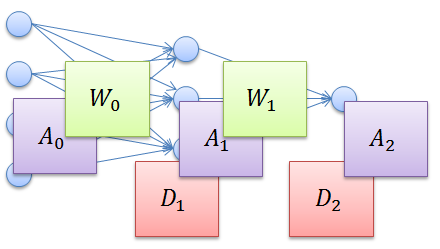
\includegraphics[width=2.4in]{gpu_neural_net_data.png}
\end{center}

\end{itemize}

\end{frame}

\begin{frame}{GPU Implementation Overview}
\begin{itemize}
\item{Training Kernels}
\begin{itemize}
\item{ Based on variants of tiled matrix multiplication }
\item{ Each thread responsible for computing a single matrix cell }
\item{ Elements are loaded into shared memory to enable data re-use }
\end{itemize}

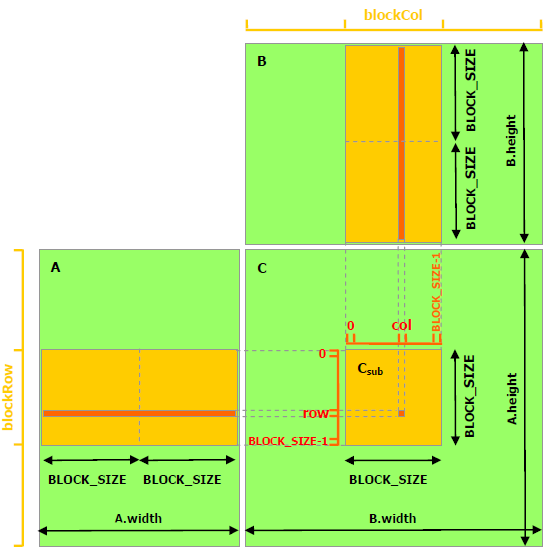
\includegraphics[width=2.0in]{matrix-multiplication-with-shared-memory.png}

\end{itemize}
\end{frame}

\begin{frame}{Data Organization \& Access}
\begin{itemize}

\item{Data Layout}
\begin{itemize}
	\item{Weight matrix is stored in row-major order}
	\item{Everything else in column-major order}
	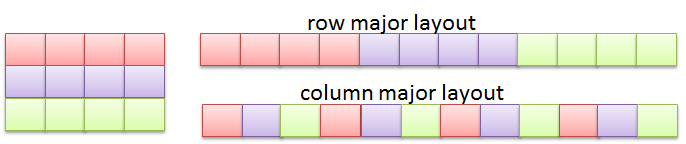
\includegraphics[width=2.4in]{gpu_data_layout.png}
\end{itemize}

\item{Global Memory Access}
\begin{itemize}
	\item{Iterate over the secondary dimension}
	\item{Row-Column matrix multiplication}
	\item{Column-Column matrix multiplication}
	
	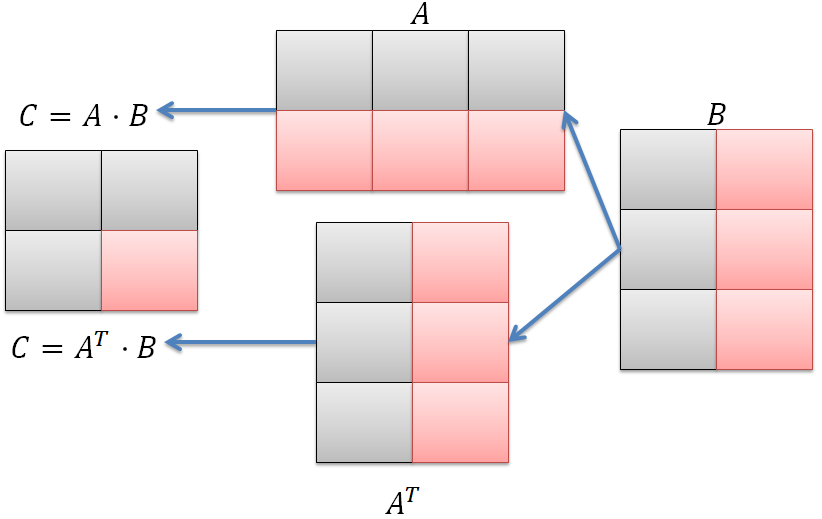
\includegraphics[width=2.2in]{gpu_mmul.png}
\end{itemize}

\end{itemize}
\end{frame}

\begin{frame}{Additional Features \& Possible Optimization}
\begin{itemize}

\item{Customizable Neural Network}
\begin{itemize}
\item{Single or double precision arithmetic}
\item{User preferred activation function}
\end{itemize}

\item{Optimization}
\begin{itemize}
\item{Minimize shared memory bank conflicts to speed up computation}


\item{Avoid recomputing the activation values for the delta matrix }
\end{itemize}

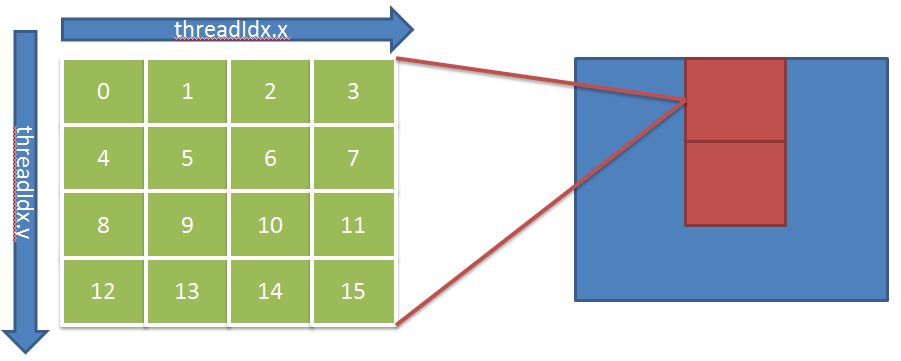
\includegraphics[width=3.0in]{gpu_mem_access.png}


\end{itemize}
\end{frame}
    


  \section{Experiments}
    \begin{frame}{MNIST dataset}
      \begin{itemize}
      \item {MNIST, handwritten digits, has a training set of 60,000 examples, and a test set of 10,000 examples.}
      \item {The digits have been size-normalized and centered in a fixed-size image to 28x28(784) image. }
      \item {10,000 examples in 60,000 training set are used as validation set and left 50,000 images are used for training.}
      \item {The original labels values are 0 to 9 but it is vectorized by one-hot encoding.}
      \end{itemize}
      \begin{center}
    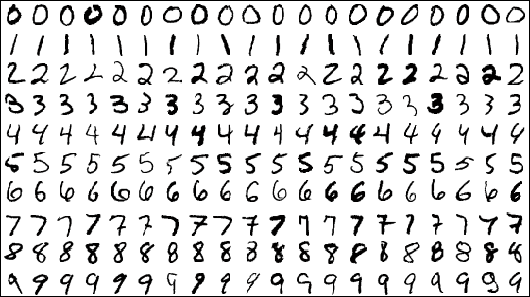
\includegraphics[width=2.4in]{mnist.png}
      \end{center}
    \end{frame}
    
\begin{frame}{Experiment parameters}
  \begin{itemize}
       \item{ \textbf{Network structures} }
				\begin{center}
				  \begin{tabular}{ | l | c | c | c | }
				    \hline
				      & \cellcolor[gray]{0.85} \# Layers & \cellcolor[gray]{0.85} \# Nodes & \cellcolor[gray]{0.85} Bias \\
				      & \cellcolor[gray]{0.85} (In,\textbf{Hidden},Out) & \cellcolor[gray]{0.85} (In,\textbf{Hidden},Out) &\cellcolor[gray]{0.85}  \\ \hline
				    Network1 & 1,\textbf{1},1 & 784,\textbf{1024},10 & Yes \\ \hline 
				    Network2 & 1,\textbf{2},1 & 784,\textbf{1024,1024},10 & Yes \\
				    \hline
				  \end{tabular}
				\end{center}
				
    \item{ \textbf{Hyperparameters} }
    \begin{center}
				  \begin{tabular}{ | c | c | c | c | }
				    \hline
				      \cellcolor[gray]{0.85} Learning Rate & \cellcolor[gray]{0.85} \# Epochs & \cellcolor[gray]{0.85} Size of Batch & \cellcolor[gray]{0.85} Regularization \\ \hline
				      0.1 & Let Me Know & $2^n$, $n\in[7,12]$ & None \\
				    \hline
				  \end{tabular}
				\end{center}
     \item{ \textbf{Activation function}}
     \begin{itemize}
      		\item{Sigmoid function}
      		\begin{align*}
      		& \sigma(z)=\frac{1}{1+e^{-z}}\\
      		& \sigma'(z)=\sigma(z)(1-\sigma(z))
      		\end{align*}
    \end{itemize}
  \end{itemize}
\end{frame}


  
  \section{Results and analysis}
\begin{frame}<beamer>{Outline}
    \tableofcontents[currentsection,currentsubsection]
  \end{frame}
 \begin{frame}{Results}
     \begin{itemize}
         \item{ \textbf{Neural Networks 1 (Net-1h)}
         }
%         \item { Accuracy is 97.78\%} 
     \end{itemize}
     
		\begin{center}
		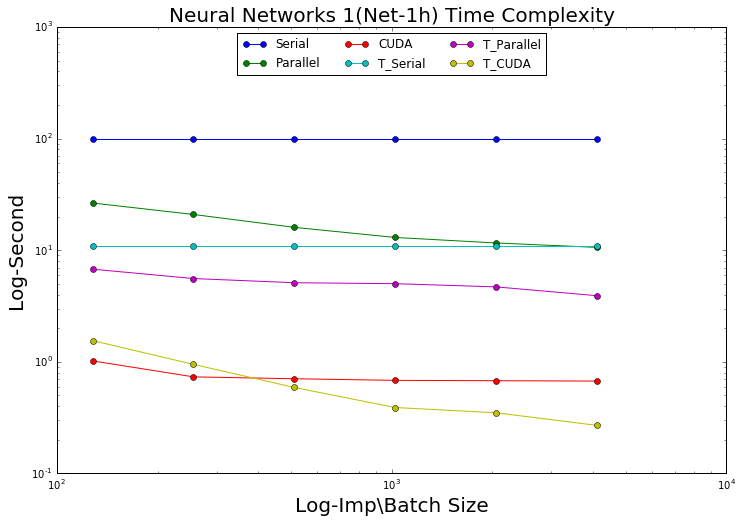
\includegraphics[width=3.4in]{nn1_time.png}
		\end{center}

 \end{frame}
 
\begin{frame}{Results (contd.)}
     \begin{itemize}
         \item{ \textbf{Neural Networks 2 (Net-2h)}
         }
%         \item { Accuracy is ???\%} 
     \end{itemize}
     
		\begin{center}
		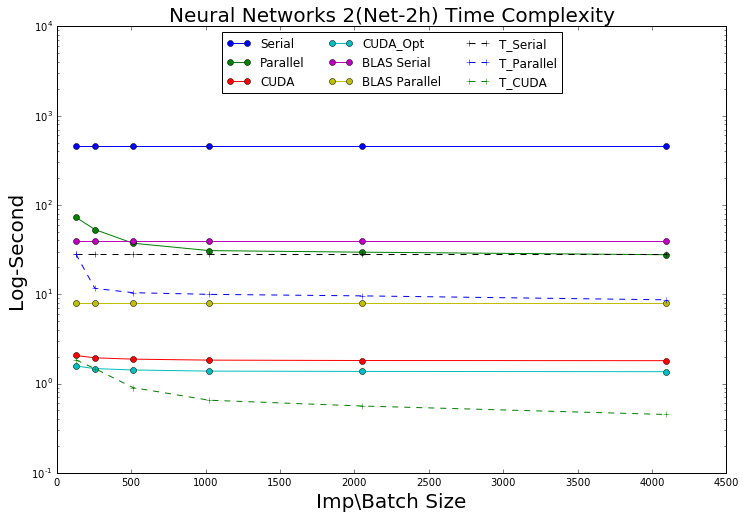
\includegraphics[width=3.4in]{nn2_time.png}
		\end{center}

 \end{frame} 

\begin{frame}{Results (contd.)}
     \begin{itemize}
         \item{ \textbf{Neural Networks 1 (Net-1h) - GFLOPS}
         }
     \end{itemize}
     
		\begin{center}
		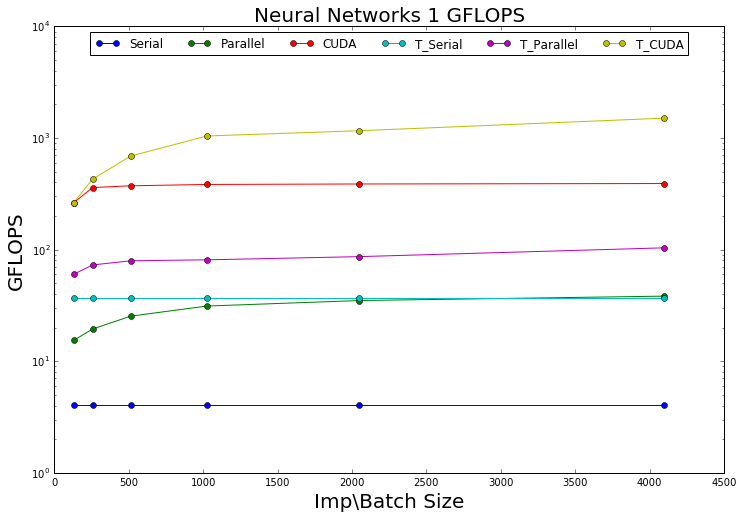
\includegraphics[width=3.4in]{nn1_gflops.png}
		\end{center}

 \end{frame} 

\begin{frame}{Results (contd.)}
     \begin{itemize}
         \item{ \textbf{Neural Networks 2 (Net-2h)- GFLOPS}
         }
     \end{itemize}
     
		\begin{center}
		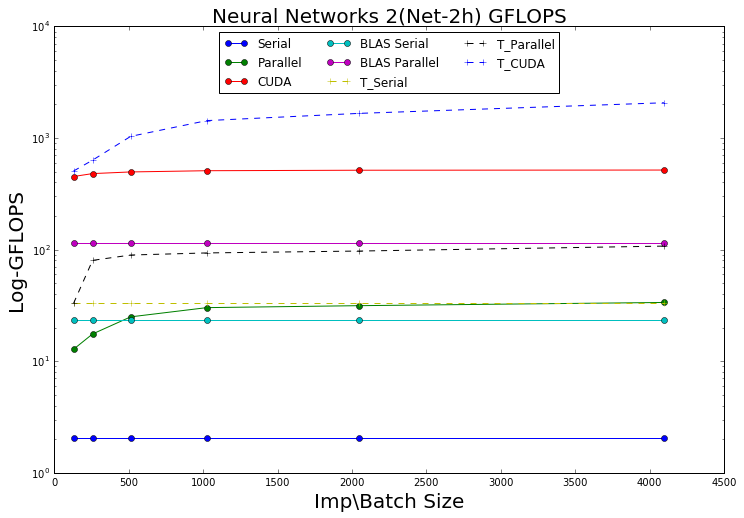
\includegraphics[width=3.4in]{nn2_gflops.png}
		\end{center}

 \end{frame} 

 
 \begin{frame}{Analysis}
 	\begin{itemize}
 	\item {Naive implementation}
 	\begin{itemize}
 	\item {Parallel computing provides faster training time than serial implementation.}
 	\item {By increasing the mini batch size, we can much faster training time.}
 	\end{itemize}
 	\item {\textbf{BLAS}}
 	\begin{itemize}
 	\item {Significantly improved results (even faster than Theano) with BLAS.}
 	\item {It is able to parallelize each Matrix-vector product.}
 	\item { This way shows that the optimized parallelism gives speed-up over Naive serial implementation.}
	\end{itemize}
	\item {\textbf{Bottlenecks}}
	\begin{itemize}
	\item {Shared memory bank conflicts reduce the parallelism.}
	\item {When the number of neurons between layers is not perfect multiple of 32 then some threads do not participate in the computation but just wait.}
	\item {As a result, it causes degraded parallelism.}
	\end{itemize}
 	\end{itemize}
 
 \end{frame}









\end{document}


